As same as last exercise the aim of this exercise is to generate the independent and continuous random variable by using the inverse transform approach and the rejection approach.

\subsection{Generated simulated value}
The first part of the exercise we generated simulated value from following distributions

1: Exponential distribution:

Let $X\sim \exp{\lambda}$ according inversion method, we have $X=F^{-1}(U)$\\
If $F(x)=1-\exp{(\lambda x)}$, then $F^{-1}(u)=-\frac{1}{\lambda}\log(1-u)$ (both 1-U and U are uniformly distributed.
\begin{equation}
    X=-\frac{\log(U)}{\lambda}\sim \exp{(\lambda)}
\end{equation}
\begin{center}
    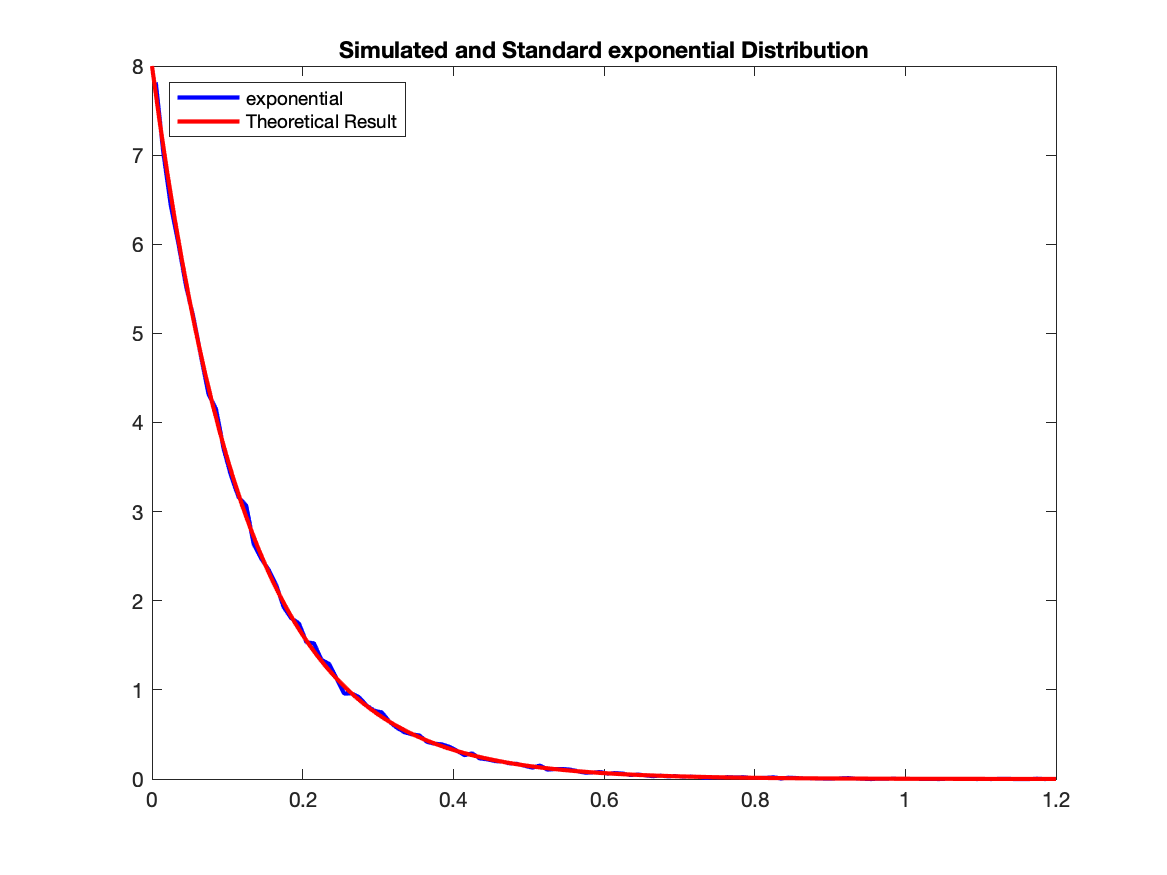
\includegraphics[scale=0.3]{Figures/figure3_1.png}\\
    \figuretitle{Figure 6: simulated values from Exponential distribution.}
\end{center}\\
\\
2: Normal distribution (at least with standard Box-Mueller):\\
Let $Z_{1},Z_{2}\sim N(0,1)$,the polar method or Box-Mueller is a way that transform from polar coordinate $\theta=2\piU_{2},r=\sqrt{-2\log(U_1)}$ into Cartesian coordinates$X=Z_{1}$ and $Y=Z_{2}$ which is given by
\begin{equation}
    Z_{1}=r\cos \theta   
\end{equation}
\begin{equation}
    Z_{2}= r\sin \theta
\end{equation}
\begin{center}
    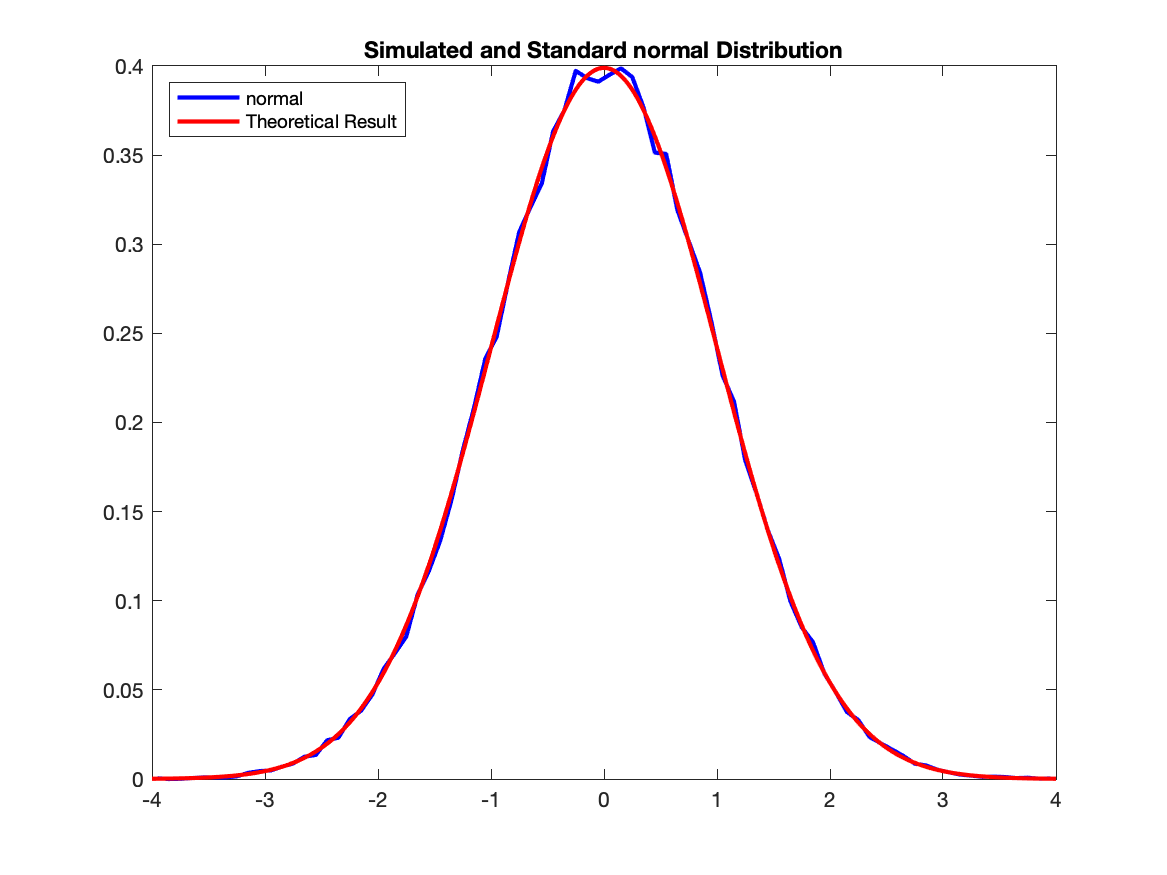
\includegraphics[scale=0.4]{Figures/figure3_2.png}\\
    \figuretitle{Figure 7: simulated values from Normal distribution.}
\end{center}\\
\\
3:Pareto distribution, with $\beta=1$ and different values of $K=2.05,2.5,3,4$\\
\begin{center}
    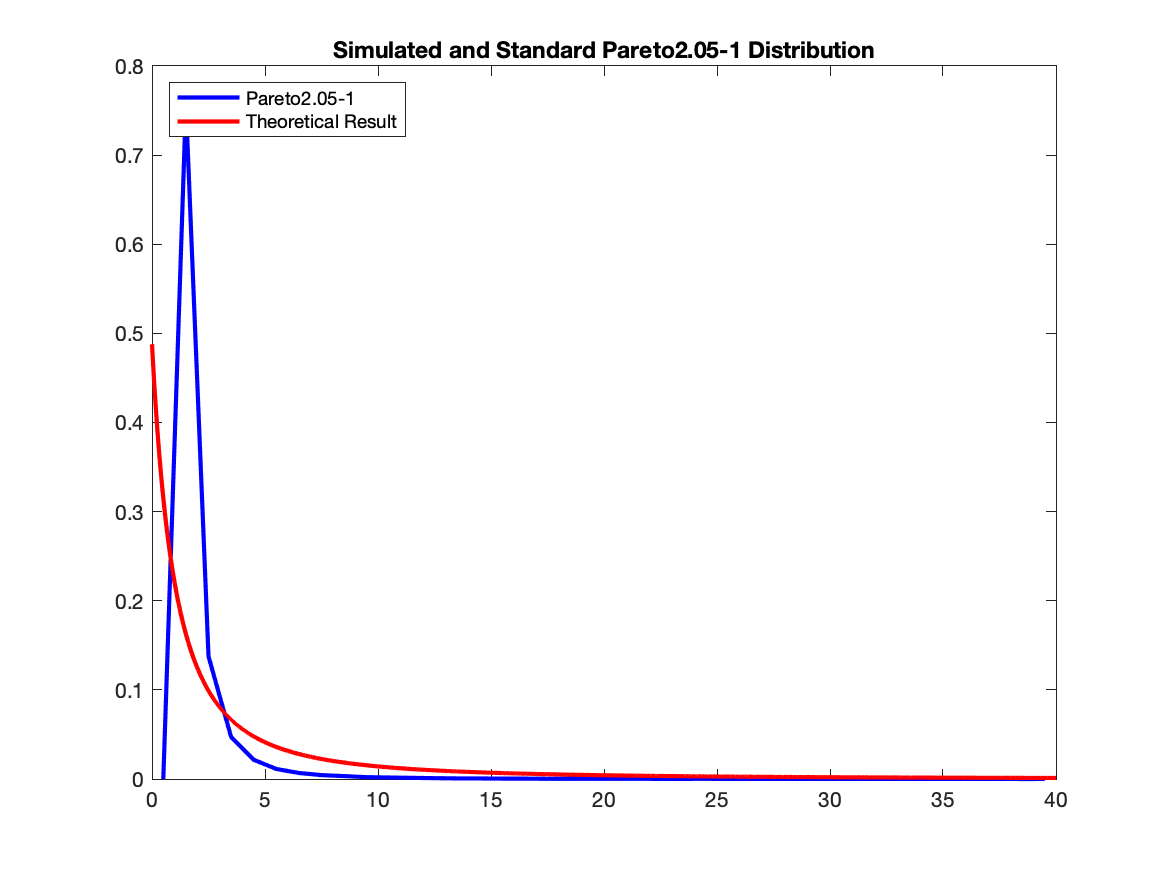
\includegraphics[scale=0.4]{Figures/figure3_3.png}\\
    \figuretitle{Figure 8: simulated values from Pareto distribution for K=2.05-1.}
\end{center}\\
\\
\begin{center}
    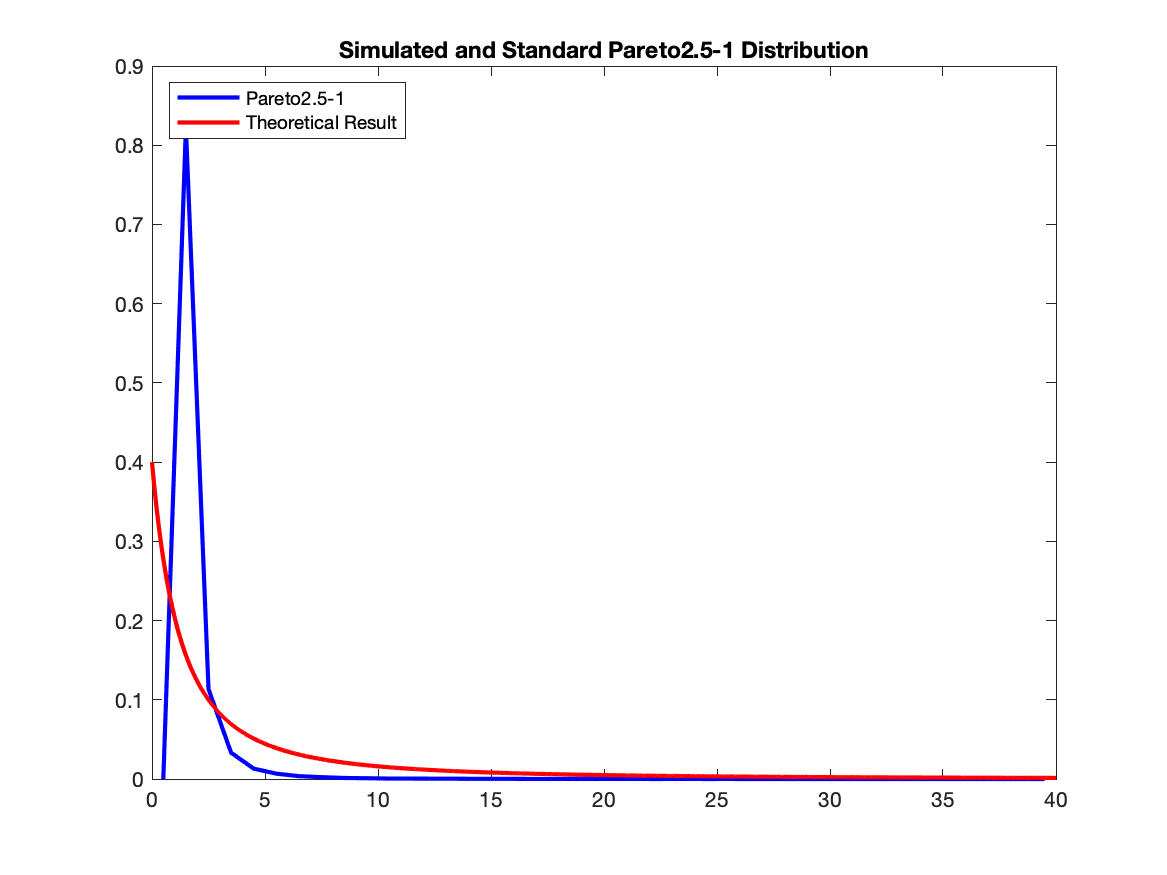
\includegraphics[scale=0.4]{Figures/figure3_4.png}\\
    \figuretitle{Figure 9: simulated values from Pareto distribution for K=2.5-1.}
\end{center}\\
\\
\begin{center}
    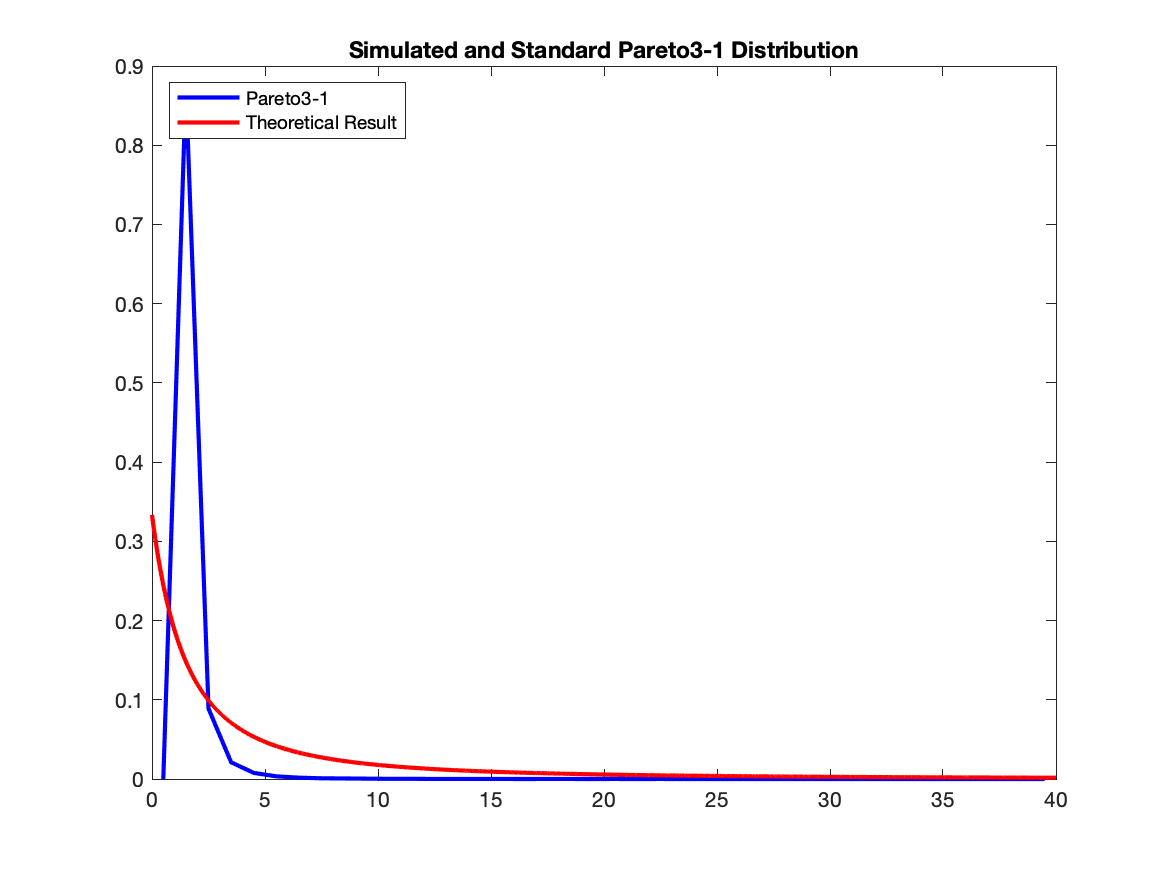
\includegraphics[scale=0.4]{Figures/figure3_5.png}\\
    \figuretitle{Figure 10: simulated values from Pareto distribution for K=3-1.}
\end{center}\\
\\
\begin{center}
    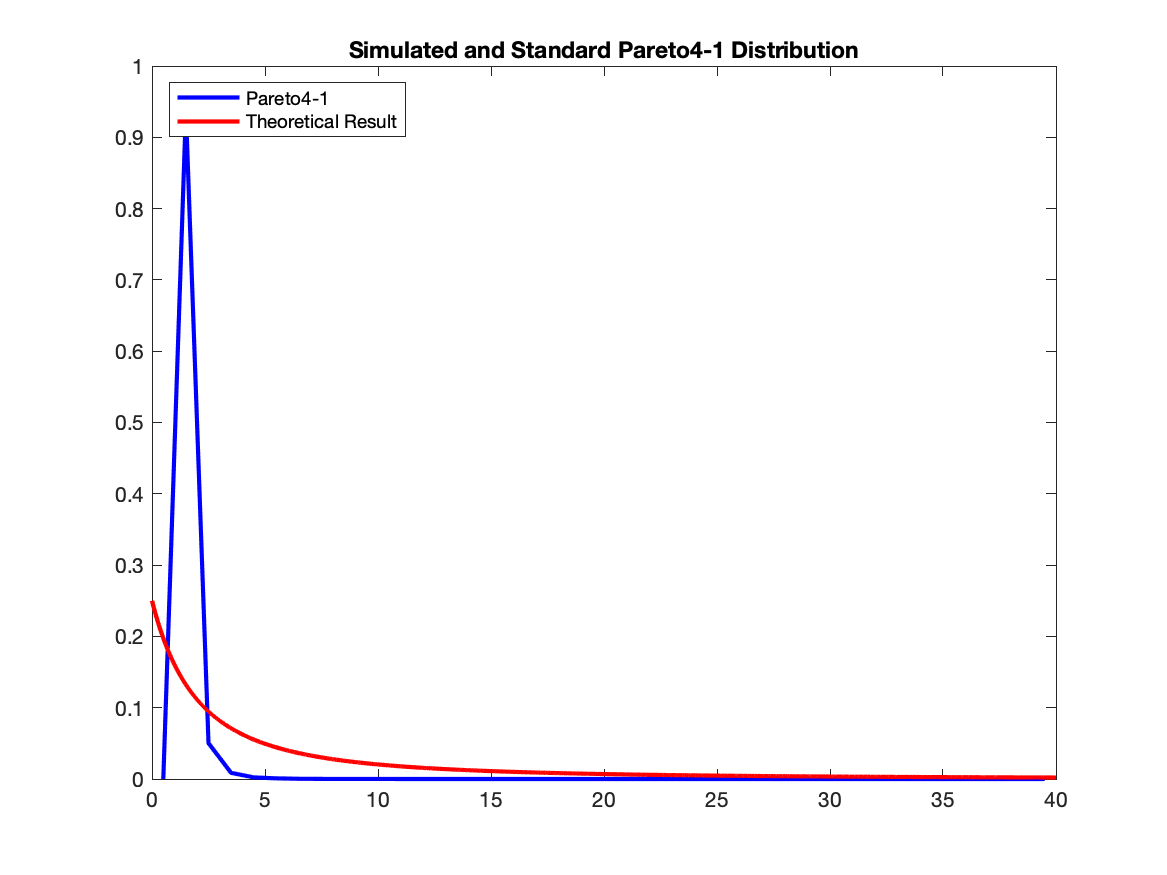
\includegraphics[scale=0.4]{Figures/figure3_6.png}\\
    \figuretitle{Figure 11: simulated values from Pareto distribution for K= 4-1.}
\end{center}\\
\\
\begin{center}
    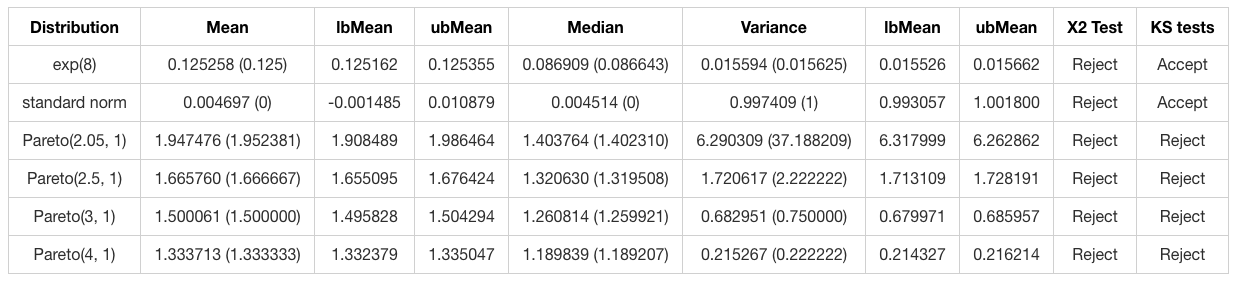
\includegraphics[scale=0.4]{Figures/figure3_7.png}\\
    \figuretitle{Table 3: Analysis and Test of the Simulation Result.}
\end{center}\\
\\







